\chapter{Data-driven background estimation}\label{chap:bkgmodel}

\section{Motivation}
An extrapolation procedure was chosen due to the broad deviations in the gradient of the mass spectrum resulting from non-resonant signatures. A fit over the full invariant mass spectrum would bais the background estimation as the background only fit would attempt to accommodate the broad deviations at high-mass. It has been shown previously by dilelpton resonance search~\cite{Aad:2019fac} and diphoton searches~\cite{Aaboud:2016tru,Aaboud:2017yyg} that the background shape can be modelled with a suitable function. The fits are constrained at the low-mass regions, where there is an abundance of statistics to provide a rigid background description. Therefore, the background model is fit in a low mass control region (CR) and the resulting fit is extrapolated to a high mass signal region (SR). An illustration of the extrapolation procedure outlining the CR and SR is shown in \cref{fig:bkgmodel:ranges}.

There are several challenges involved with the extrapolation approach. One challenge involves the choice of function picked to model the fit in the low-mass control region and the high mass extrapolation. A central part in the analysis is quantifying the bias introduced by the choice of a particular function as an uncertainty and the uncertainty on both the shape and normalisation of the extrapolated background. The choice of CR and SR effect the sensitivity, therefore they are optimised to maximise the expected sensitivity. The choice of function, CR and SR, and estimation of uncertainties are described in the chapters below. All fits are performed within the RooFit~\cite{RooFit} framework.

\begin{figure}[!htpb]
    \centering
    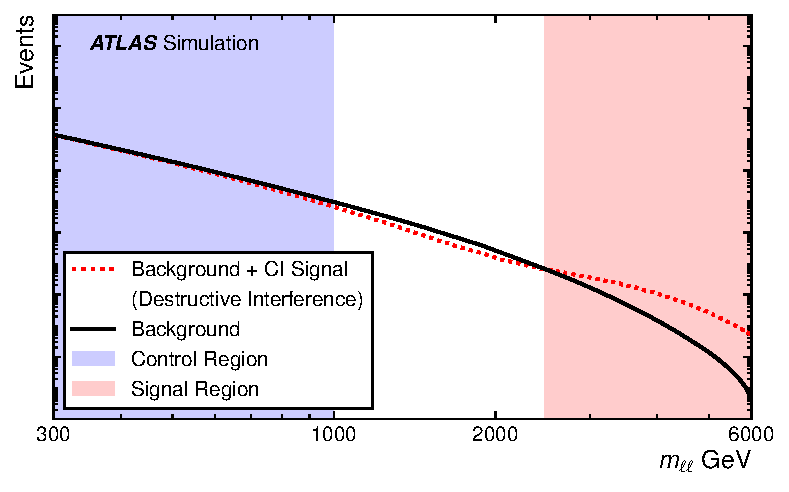
\includegraphics[width=0.8\textwidth]{/Users/Deshan/Documents/PhD/thesis/Thesis/figures/analysis/bkgmodel/fig_01a.pdf} 
    \caption[A schematic illustration of the possible mass ranges in this analysis.]{A schematic illustration of the possible mass ranges in this analysis.
    The monotonically falling total background shape is shown by the solid black line, while an example of a CI signal plus the total background shape is shown by the dotted red line. The CI signal is shown after the DY process has been subtracted to show only the interference and pure CI process. The gap illustrated between the CR and the SR is found to be the preferred case for the destructive interference cases only.}
    \label{fig:bkgmodel:ranges}
\end{figure}

\section{Background function choice}\label{sec:modelchoice}
The functional form used to fit the background was chosen from a variety of different candidates for it's stability during the extrapolation procedure and it's ability to model the invariant mass distributions of the \ee and \mumu channels. Each function is fit to the background dilepton invariant mass template, produced by summing together the contributions from all the background processes, in a variety of different CRs and extrapolated to the corresponding SRs. The pulls, defined as (fit-simulation)/$\sqrt{\mathrm{fit}}$, for each invariant mass bin if obtained, and the function resulting in pulls below two is kept. Additionally, the function with the best $\chi^2$ in the CR is selected.

The function that best satisfies the criteria is given in \cref{eq:fitfunc}. The same function was used in the dilepton heavy resonance analysis~\cite{Aad:2019fac}.
\begin{equation}
    \label{eq:fitfunc}
    \begin{aligned}
        & f_\textrm{b}(m_{\ell\ell}) = f_{\mathrm{BW},Z}(m_{\ell\ell}) \cdot \left(1 - x^{c}\right)^{b} \cdot x^{\sum_{i=0}^3 p_i\log(x)^i}, \\
        & f_{\mathrm{BW},Z}(\mathrm{m_{\ell\ell}}) = \frac{\Gamma_Z}{(m_Z - \mathrm{m_{\ell\ell}})^2 + \Gamma_Z^2},
    \end{aligned}
\end{equation}
where $x = m_{\ell\ell}/\sqrt{s}$. The first term, $f_{\mathrm{BW},Z}(m_{\ell\ell})$, is a non-relativistic Breit--Wigner function with $m_Z = \SI{91.1876}{\giga\electronvolt}$ and $\Gamma_Z = \SI{2.4952}{\giga\electronvolt}$~\cite{PhysRevD.98.030001}. The $(1 - x^{c})$ ensures that the background fit evaluates to zero as $x \to 1$, to be consistent with the expectation from the collision energy of the LHC. Both b and c are chosen to be fixed based on fits to the full background template. The $p_i$ parameters, with $i = 0,..,3$, are left as free parameters to be informed by the fit. 

The fits to the data and simulation are both performed with bin width of \SI{1}{\giga\electronvolt}. The function $f_b(m_{\ell\ell})$ is treated as probability density in the fits performed to the CR, and normalised in the CR to the number of events in the CR ($N_{CR}$) of the template being fit. \cref{fig:bkgmodel:fitstoMC} shows an example of background only fits to the electron and muon channel in a CR and SR configuration. The binning of the plots were changed to be constant in $\log{(\text{m}_{\ell\ell})}$ from 230--\SI{6000}{\giga\electronvolt} for the purposes of presentation, as figures with the linear \SI{1}{\giga\electronvolt} binning will be difficult to interpret clear. In \cref{fig:bkgmodel:fitstoMC2} some disagreement between in the fit and the and the background template can be seen when extrapolated to high mass, however, the difference  corresponding number of events between the extrapolation and background template will be very small in the single-bin SR. 

\begin{figure}[h!]
    \centering
    \begin{subfigure}[b]{0.49\textwidth}
        \centering
        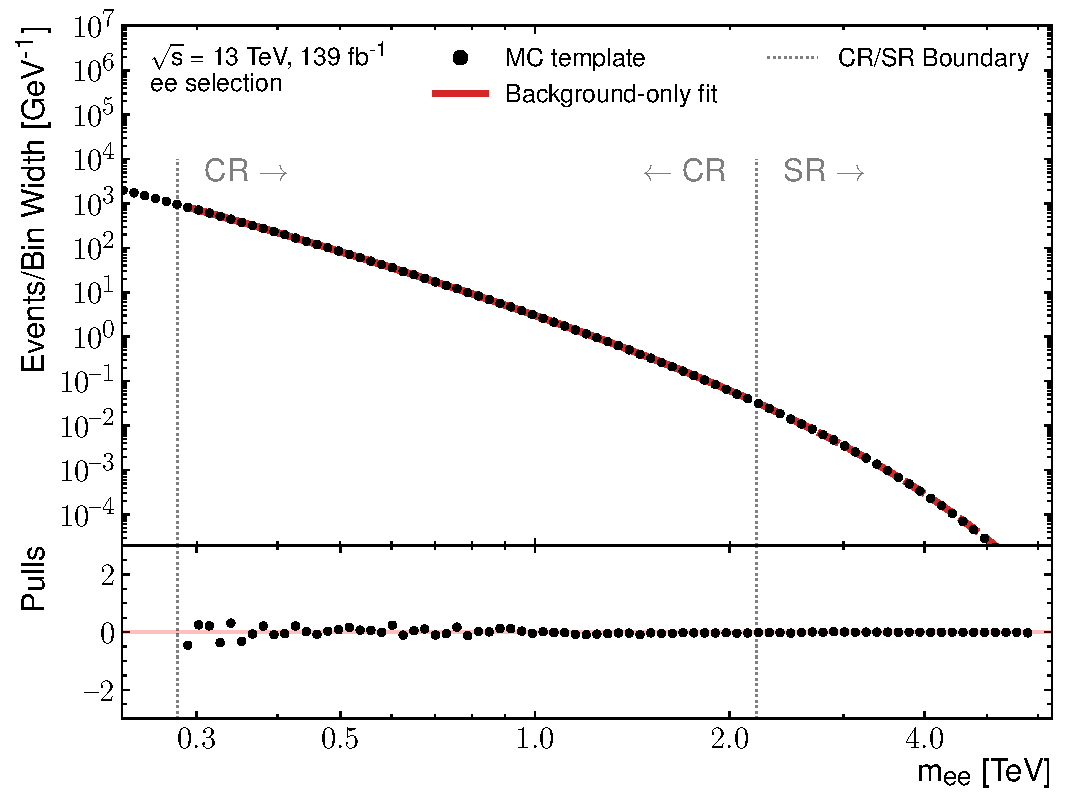
\includegraphics[width=\textwidth]{/Users/Deshan/Documents/PhD/thesis/Thesis/figures/analysis/bkgmodel/fit-const-ee-backgroundModel.pdf}
        \label{fig:bkgmodel:fitstoMC1}
    \end{subfigure}
    \begin{subfigure}[b]{0.49\textwidth}
        \centering
        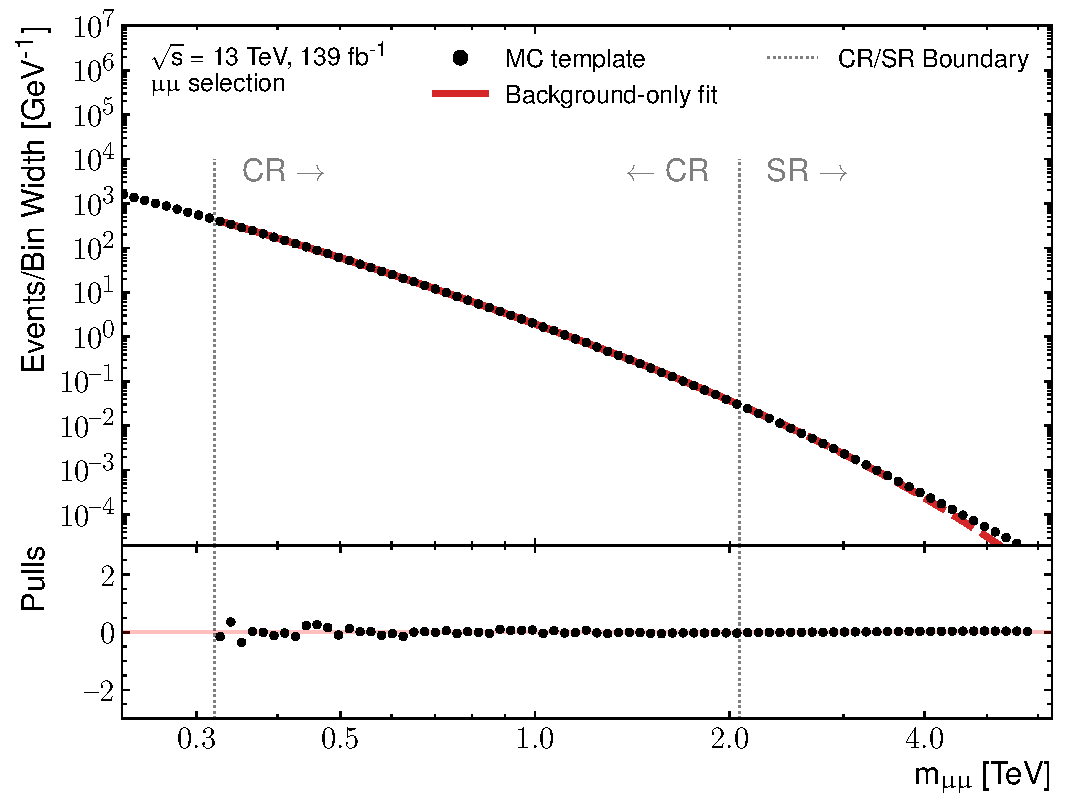
\includegraphics[width=\textwidth]{/Users/Deshan/Documents/PhD/thesis/Thesis/figures/analysis/bkgmodel/fit-const-mm-backgroundModel.pdf}
        \label{fig:bkgmodel:fitstoMC2}
    \end{subfigure}
    \caption[Fits to the simulated background template in the electron and muon channels]{fit to the simulated background template in the electron (left) and muon (right) channels shown in the top pad. The bottom pad shows the pulls of the fit. The CR and SR boundaries are also shown in the figure. The background template points are plotted at the centre of each bin as the number of events divided by the bin width, which is constant in $\log{(\text{m}_{\ell\ell})}$.}
    \label{fig:bkgmodel:fitstoMC}
\end{figure}

Examples of functions that did not satisfy the above criteria are given in \cref{tab:bkgmodel:functions}, with their corresponding fits to the data shown in \cref{fig:bkgmodel:badfitstomc}. Nonphysical behaviour in the fit and  extrapolation can be seen in \cref{fig:bkgmodel:fitstoMC5}. \cref{fig:bkgmodel:fitstoMC4,fig:bkgmodel:fitstoMC6} were not selected due to poor modelling of the CR. \cref{fig:bkgmodel:fitstoMC3} depicts a function fit that is close to satisfying the function choice selection, however, it poorly models the extrapolated region compared to the function defined in \cref{eq:fitfunc}.

\begin{table}[h!]
    \centering
    \begin{tabular}{c|l}
         & Function definition \\
        \hline\hline 
        1 & $(1 - x^{5})^{\text{p0}}*(x^{(\text{p1} + \text{p2}*\log(x)})$ \\
        2 & $(1-\log(e*x^{\text{p1}})+c1*x*e^{\text{p2}/(1+x^{\text{p3}})}$ \\
        3 & $(x)^{\text{p1}}*e^{\text{p2}*x}$\\
        4 & $(1-x)^{\text{p1}}*e^{\text{p2}*x^2}$ \\
	\end{tabular}
    \caption[List of functions considered for the background fit]{List of functions considered for fit to dilepton spectrum that did not pass the criteria required. $x$ is defined to be $= m_{\ell\ell}/\sqrt{s}$. }
    \label{tab:bkgmodel:functions}
\end{table}

\begin{figure}[h!]
    \centering
    \begin{subfigure}[b]{0.49\textwidth}
        \centering
        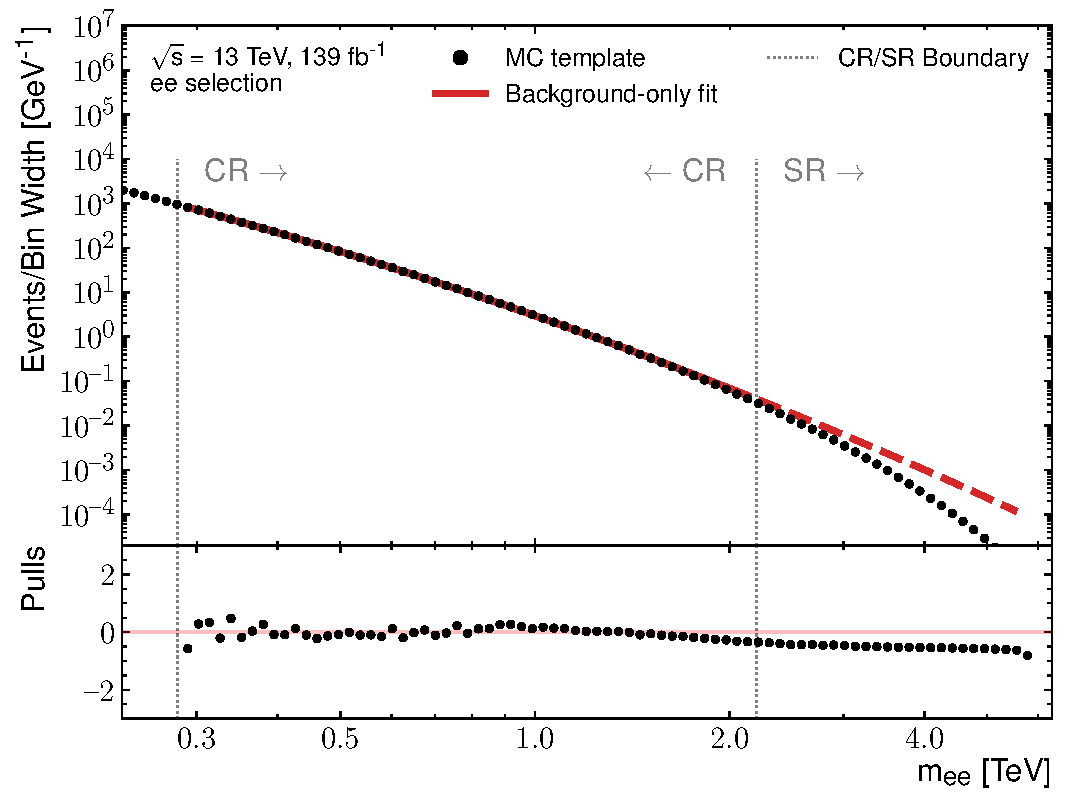
\includegraphics[width=\textwidth]{/Users/Deshan/Documents/PhD/thesis/Thesis/figures/analysis/bkgmodel/fit-const-ee-diphoton3.pdf}
        \caption{}
        \label{fig:bkgmodel:fitstoMC3}
    \end{subfigure}
    \begin{subfigure}[b]{0.49\textwidth}
        \centering
        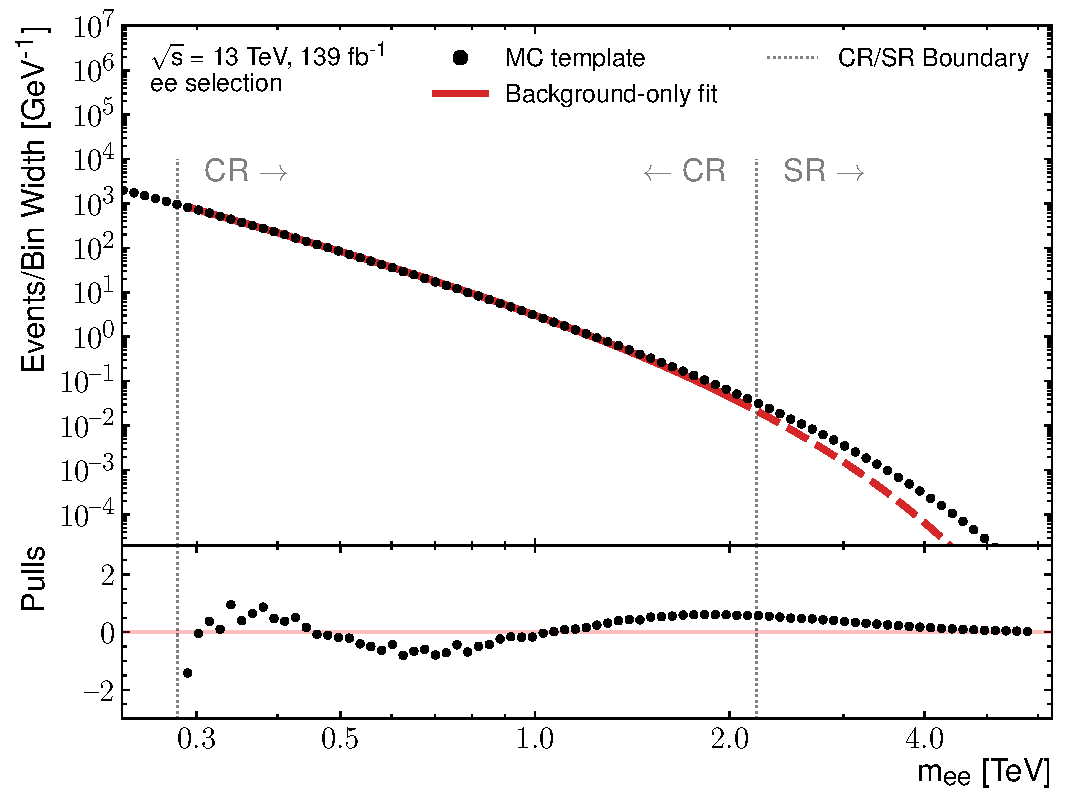
\includegraphics[width=\textwidth]{/Users/Deshan/Documents/PhD/thesis/Thesis/figures/analysis/bkgmodel/fit-const-ee-dext1.pdf}
        \caption{}
        \label{fig:bkgmodel:fitstoMC4}
    \end{subfigure}
    \begin{subfigure}[b]{0.49\textwidth}
        \centering
        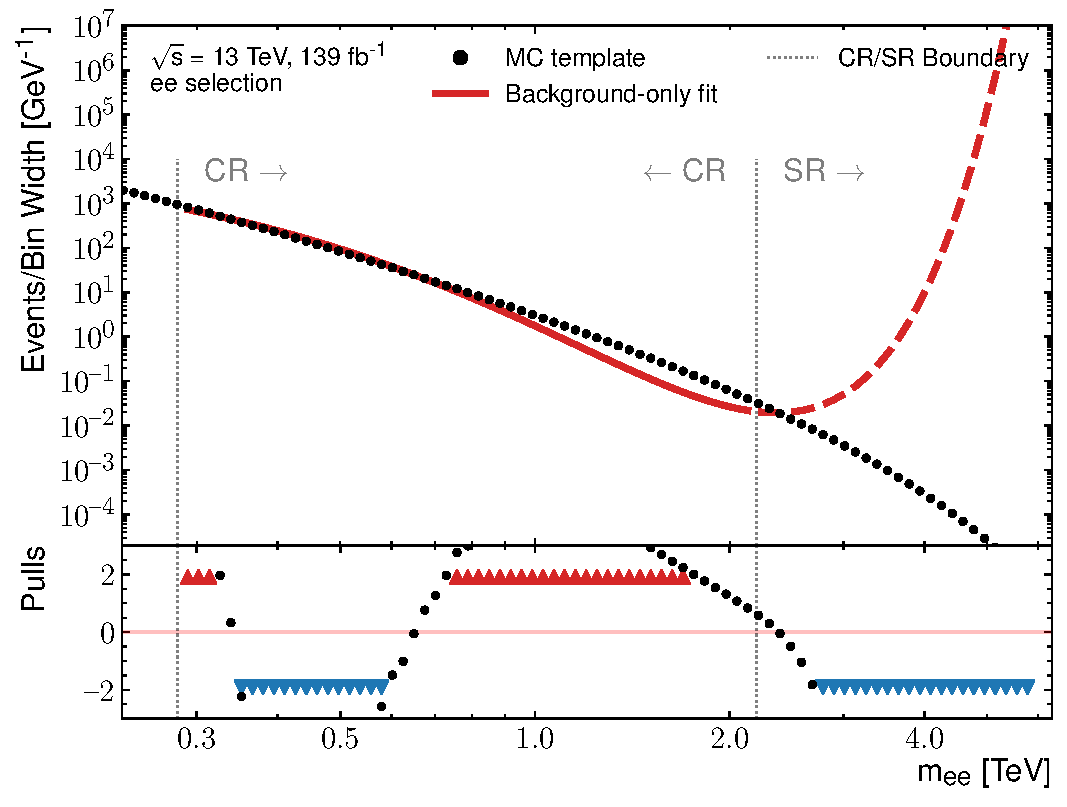
\includegraphics[width=\textwidth]{/Users/Deshan/Documents/PhD/thesis/Thesis/figures/analysis/bkgmodel/fit-const-ee-multijetf2.pdf}
        \caption{}
        \label{fig:bkgmodel:fitstoMC5}
    \end{subfigure}
    \begin{subfigure}[b]{0.49\textwidth}
        \centering
        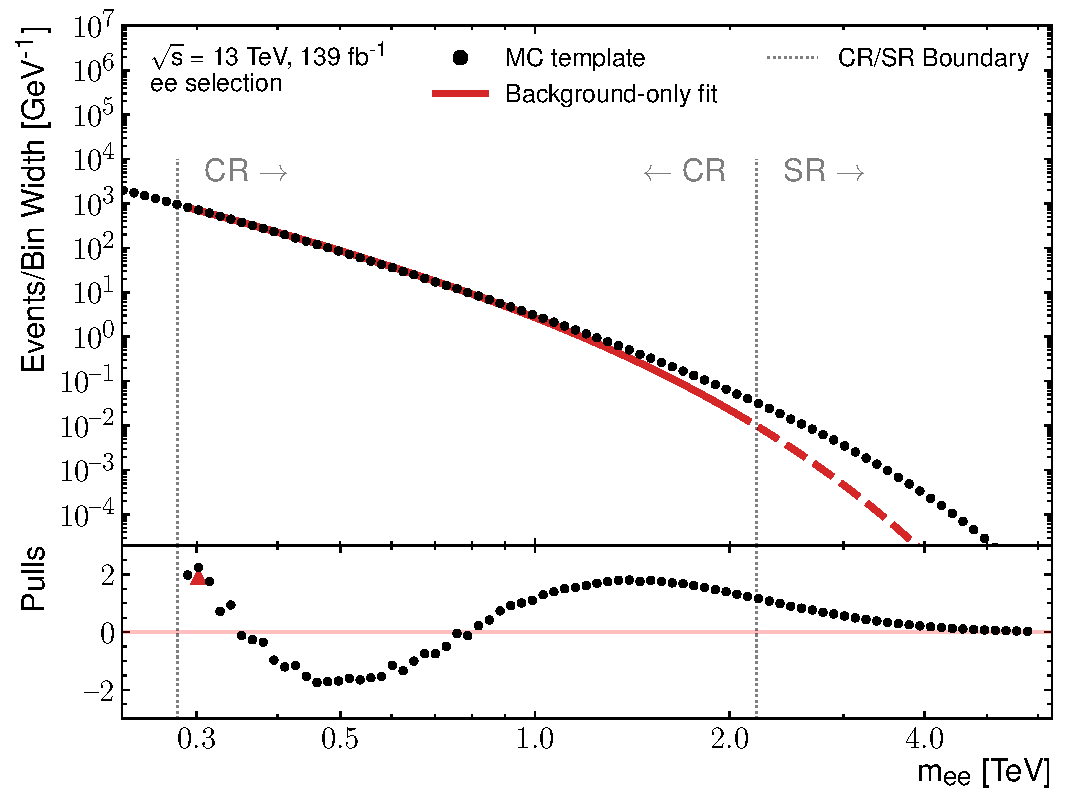
\includegraphics[width=\textwidth]{/Users/Deshan/Documents/PhD/thesis/Thesis/figures/analysis/bkgmodel/fit-const-ee-UA2_1.pdf}
        \caption{}
        \label{fig:bkgmodel:fitstoMC6}
    \end{subfigure}
    \caption[Fits to the simulated background template in the electron and muon channels using functions that did not pass the selection criteria]{Fits using functions that failed the function choice criteria, to the simulated background template in the electron channel shown in the top pad. Figures (a), (b), (c) and (d) correspond to functions 1, 2, 3, and 4 in \cref{tab:bkgmodel:functions}, respectively. The bottom pad shows the pulls of the fit. The CR and SR boundaries are also shown in the figure. The background template points are plotted at the centre of each bin as the number of events divided by the bin width, which is constant in $\log{(\text{m}_{\ell\ell})}$.}
    \label{fig:bkgmodel:badfitstomc}
\end{figure}

\section{Signal model}\label{sec:sigmodel}
To avoid bais from possible signal contamination in the CR, the CR region choice is validated using a signal+background model, where signal injection tests are performed in each of the CR and SR region configurations. A collection of signal+background distributions are produced by simulation for various $\Lambda$ values of interest. A signal component is added to \cref{eq:fitfunc} to fit the signal+background distributions, defined as: 
\begin{equation}
    \label{eq:sbfunction}
    \begin{aligned}
    f_\textrm{b+s}(m_{\ell\ell},\Lambda) = N_\textrm{b}\cdot f_\textrm{b}(m_{\ell\ell}) + N_\textrm{s}(\Lambda)\cdot f_\textrm{s}(m_{\ell\ell},\Lambda),
    \end{aligned} 
\end{equation}
where $f_\textrm{s}(m_{\ell\ell},\Lambda)$ is the signal probability density function and $N_\textrm{s}(\Lambda)$ is the number of signal events in the CR. Both $f_\textrm{s}(m_{\ell\ell},\Lambda)$ and $N_\textrm{s}(\Lambda)$ are determined from simulation. The morphing procedure, described in \cref{sec:datamc:mc:sig:morphing} is used to obtain a smooth descriptions of a given CI model as function of $\Lambda$, which allows to determine signal contributions that fall between the fixed signal shapes from simulation. The parameter $N_\textrm{b}$ is the number of background events in the CR with the constraint $N_\textrm{b}+N_\textrm{s}(\Lambda)=N_\textrm{CR}$.  

\cref{fig:bkgmodel:sbfits} depicts signal+background fits to a background template injected with a CI interaction signal at $\Lambda = \SI{26}{\tera\electronvolt}$ in the electron and muon channels. The background component of the signal+background fit is separated and compared with the background template and the pulls are calculated. The figure shows the background component of the signal+background fits are not biased by the presence of signal in the control region. 

\begin{figure}[h!]
    \centering
    \begin{subfigure}[b]{0.49\textwidth}
        \centering
        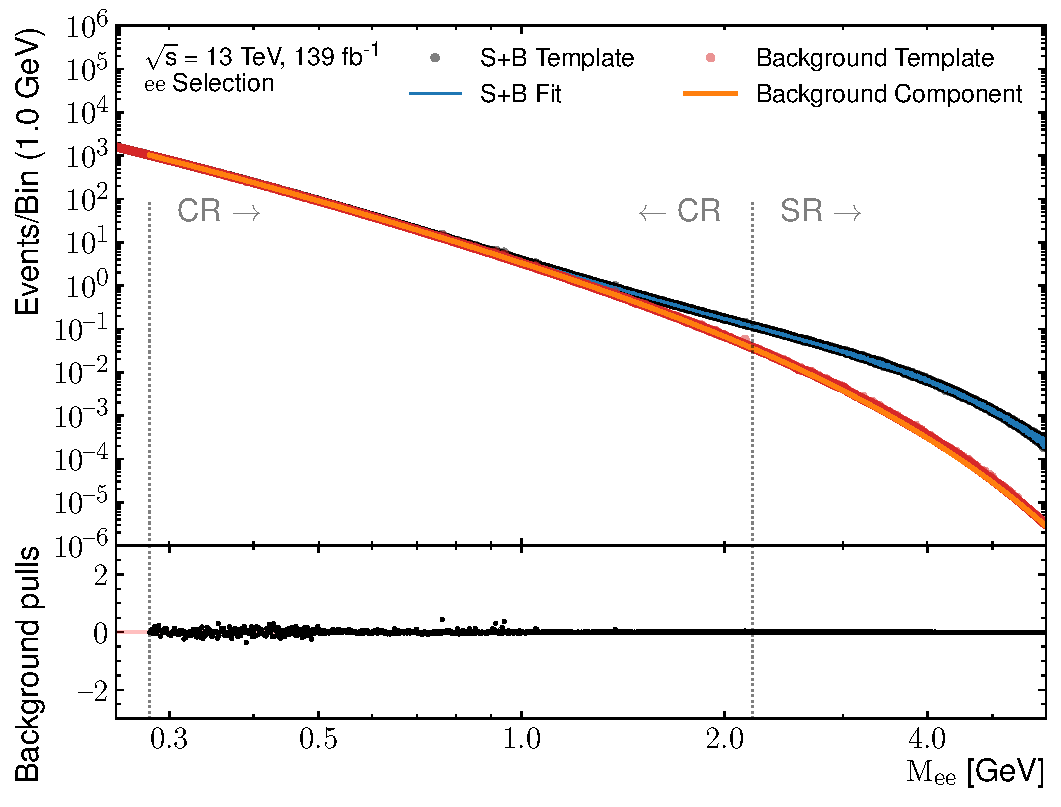
\includegraphics[width=\textwidth]{/Users/Deshan/Documents/PhD/thesis/Thesis/figures/analysis/bkgmodel/nominalFit-sb-const-LL-18-sbTrue-ee-.pdf}
        \label{fig:bkgmodel:sbfits1}
    \end{subfigure}
    \begin{subfigure}[b]{0.49\textwidth}
        \centering
        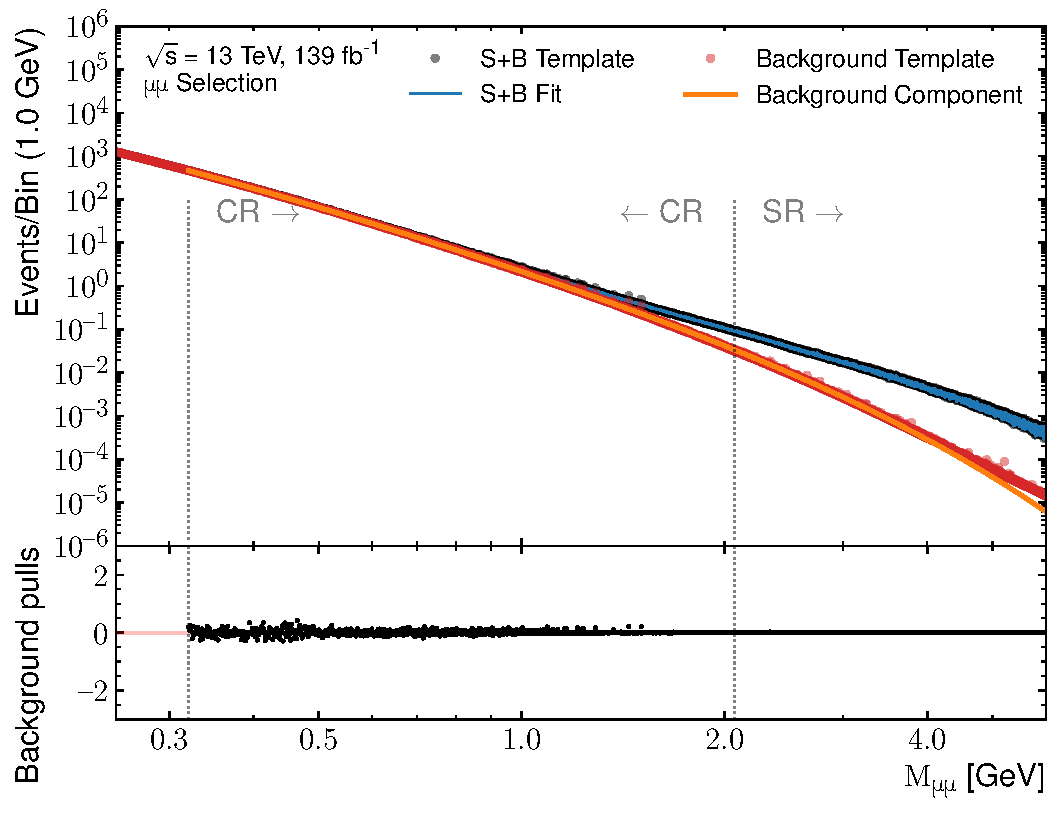
\includegraphics[width=\textwidth]{/Users/Deshan/Documents/PhD/thesis/Thesis/figures/analysis/bkgmodel/nominalFit-sb-const-LL-18-sbTrue-mm-.pdf}
        \label{fig:bkgmodel:sbfits2}
    \end{subfigure}
    \caption[Signal+Background fits to the signal+background template in the electron and muon channels]{Signal+background (S+B) fit to the simulated template injected with a CI signal at $\Lambda = \SI{26}{\tera\electronvolt}$ in the electron (left) and muon (right) channels shown in the top pad. The background template and the background component of the S+B fit is also shown. The bottom pad shows the pulls of the background component of the fit compared to the background template. The CR and SR boundaries are shown in the figure.}
    \label{fig:bkgmodel:sbfits}
\end{figure}

\subsection{Validation of the control region}
The robustness of the background estimate resulting from the fit to the final CR configuration chosen is tested. The background estimate resulting from the background only fit and extrapolation for a given CR and SR region configuration is required to be unaffected by the possible contamination of a signal in the CR. Therefore, the signal+background model is used to validate the background only fit and CR choice. The tests are performed on data once a CR and SR region choice has been chosen following the procedure described in \cref{sec:extrap:optimisation}. 

For a given CR both the background only and signal+background functions are fit and the background only components of the signal+background fit is compared to the background only model. If the two background estimates do not differ significantly, then it can be concluded that there is no significant signal contribution present in the CR to bias the background only fit. A difference greater than uncertainty on the background estimate from the signal+background fit is considered to be large enough to invalidate a CR choice. Both in the presence and absence of signal, the background component of the signal+background fits are not deflected significantly. 

If a significant difference is observed between the two background estimates, then it is concluded that the control region includes an invariant mass range where a signal can impact the background only fit. Due to the expected the shape of the CI signals, the bias from the signals are a consequence the CR extending into high-mass regions where the CI signals start to dominate. Therefore, the CR upper edge can be lowered iteratively, each time checking the background estimates from the two fit functions, until they agree. A large difference between the background estimates from the two fit functions is only expected in data only if there is a CI or other non-resonant signal present. 

An example test of the compatibility of the signal+background and background only fits is shown in \cref{fig:bkgmodel:fitsbplusb}. The integrated number of background events in the SR from each fit is shown for a CR and SR configuration. The fits are performed on data once the CR and SR choices have been finalised. This example depicts a good agreement between the two fit models. The uncertainty shown corresponds to the uncertainty on the background estimate from the signal+background fit. Any difference observed between the two background estimates will be used as an additional uncertainty on the background estimate. Further detail on the estimation of background model uncertainties are given in \cref{sec:extrap:uncertainties}. 

The background estimate resulting from the two fit models fitting a data with an injected signal in an invalid CR choice is shown in \cref{fig:bkgmodel:fitsbplusbbad}. A CI signal corresponding to $\Lambda = \SI{18}{\tera\electronvolt}$ has been injected into the data and CR region moved into high mass to exaggerate the effects on the background estimate. The background estimate from the background only fit is significantly deflected due an excess of signal events in the CR.

\begin{figure}[h!]
    \centering
    \begin{subfigure}[b]{0.49\textwidth}
        \centering
        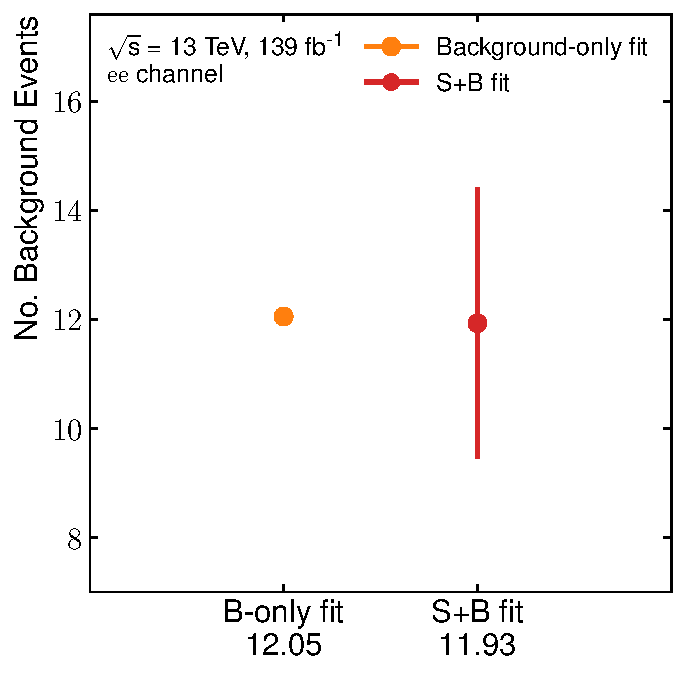
\includegraphics[width=\textwidth]{/Users/Deshan/Documents/PhD/thesis/Thesis/figures/analysis/bkgmodel/nbkg-LL-const-ee.pdf}
        \label{fig:bkgmodel:fitsbplusb1}
    \end{subfigure}
    \begin{subfigure}[b]{0.49\textwidth}
        \centering
        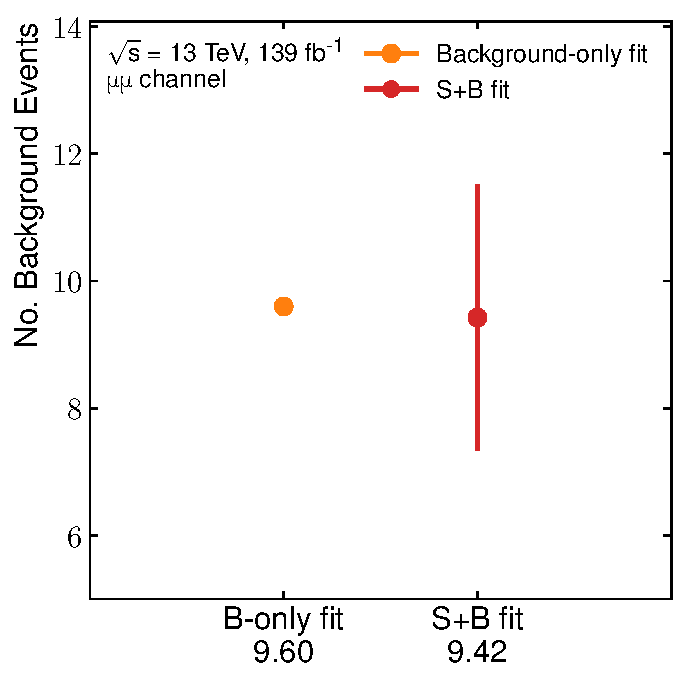
\includegraphics[width=\textwidth]{/Users/Deshan/Documents/PhD/thesis/Thesis/figures/analysis/bkgmodel/nbkg-LL-const-mm.pdf}
        \label{fig:bkgmodel:fitsbplusb2}
    \end{subfigure}
    \caption[Background estimation comparisons of the signal+background fit and background only fit]{Number of background events in the signal region from the background only fit and the signal+background (S+B) fit on data for the electron channel (left) and muon channel (right). The uncertainty on the background estimate is shown for background only fit. The number of background events from each fit is shown on the x-axis.}
    \label{fig:bkgmodel:fitsbplusb}
\end{figure}

\begin{figure}[h!]
    \centering
    \begin{subfigure}[b]{0.49\textwidth}
        \centering
        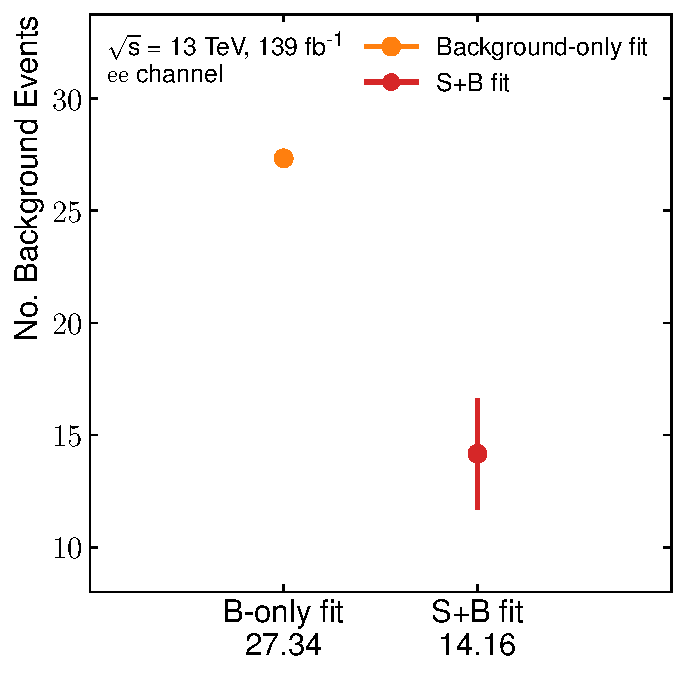
\includegraphics[width=\textwidth]{/Users/Deshan/Documents/PhD/thesis/Thesis/figures/analysis/bkgmodel/nbkg-LL-const-ee-bad.pdf}
        \label{fig:bkgmodel:fitsbplusb1bad}
    \end{subfigure}
    \begin{subfigure}[b]{0.49\textwidth}
        \centering
        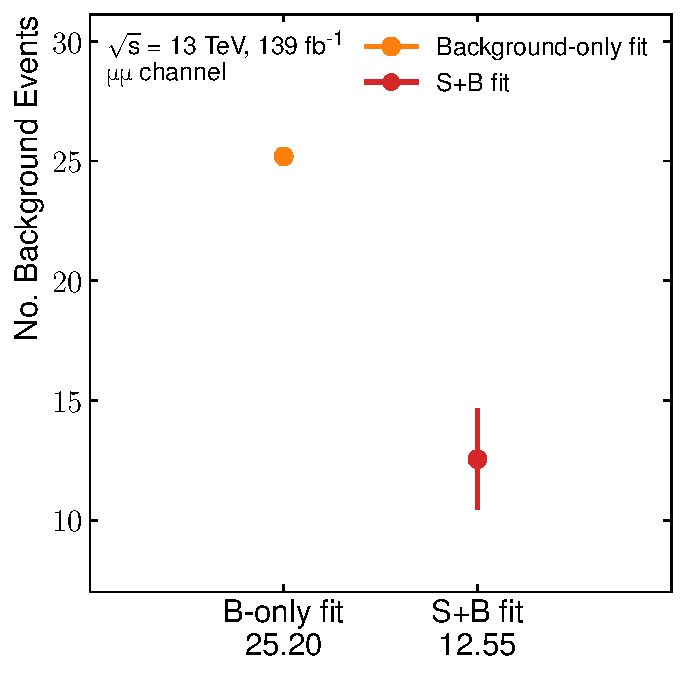
\includegraphics[width=\textwidth]{/Users/Deshan/Documents/PhD/thesis/Thesis/figures/analysis/bkgmodel/nbkg-LL-const-mm-bad.pdf}
        \label{fig:bkgmodel:fitsbplusb2bad}
    \end{subfigure}
    \caption[Background estimation comparisons of the signal+background fit and background only fit in an invalid CR choice.]{Number of background events in the signal region from the background only fit and the signal+background (S+B) fit on data with an injected CI signal with $\Lambda = \SI{18}{\tera\electronvolt}$, for the electron channel (left) and muon channel (right). The uncertainty on the background estimate is shown for background only fit. The number of background events from each fit is shown on the x-axis.}
    \label{fig:bkgmodel:fitsbplusbbad}
\end{figure}

\section{Uncertainties}\label{sec:extrap:uncertainties}

\section{Optimisation of control and signal regions}\label{sec:extrap:optimisation}


